\chapter{研究方案及步骤}

\begin{figure}[!htbp]
    \begin{center}
        
    \end{center}
    \caption{研究方案流程图}
\end{figure}

\section{配方设计原则}
CPVC 润滑体系与热稳定体系采用控制变量法进行配方设计,配方的基本组成如表 \ref{tab2} 所示

\begin{table}[!htbp]
    \caption{CPVC 基本配方设计表}
    \label{tab2}
    \begin{center}
    \footnotesize{
        \begin{tabular}{ccccccc}
            \Xhline{1pt}
            CPVC & 抗冲击改性剂 & 热稳定剂\footnotemark[1] & 外润滑剂\footnotemark[2] & 内润滑剂\footnotemark[3] & 加工助剂 & 钛白粉 \\
            \Xhline{0.5pt}
            100\footnotemark[4] & 8 & 2 & 1.3 & 1.2 & 3 & 2   \\
            \Xhline{1pt}
        \end{tabular}
    }
    \end{center}
\end{table}
\footnotetext[1]{包括有机锡(TMG-234)、有机锡(实验室)、液体有机锡}
\footnotetext[2]{包括 AC-316、AC-617、AC-629、PEW-0380、A 蜡、OP 蜡}
\footnotetext[3]{包括汉高 G-60、OA2 蜡、E 蜡}
\footnotetext[4]{均表示份数}

\section{制样流程}

\subsection{混料}
配混料混合效果的好坏将直接影响制品的均匀性与力学性能,因而该步采用高速混合机进行原料的混合。\par
按配方准确称量各助剂,将 CPVC 树脂及各助剂按煞有顺序加入到高速混合机中,混合 3 分钟制成配混料。为防止因摩擦生热使得 CPVC 发生热分解,采用每搅拌 2 s 暂停 3 s 的间歇式搅拌方法,控制在较低的温度。

\subsection{塑化开炼}
该步是将制得的配混料加入到双辊开炼机中,通过控制两个辊筒的转速比使得物料受到剪切作用,从而达到塑炼的混合效果。\par
通过对 CPVC 玻璃化转变温度 $T_g$ 与热分解温度 $T_d$ 的参考,将双辊开炼机的辊温设定为 190\cd。将配混料加入到开炼机中反复进行塑化开炼,塑化时间约 5 min。

\subsection{压片}
在 180\cd、10 MPa 条件下,采用平板硫化机热压 3 min 左右,重复开合压板排气 4$\sim$5 次,再冷压 5 min 即得到待测试样片。

\subsection{切割}
按照最终性能测试的要求,将样片切割成标准样条。


\section{表征方法}
对标准样条进行力学、热学、断面形貌等性能的测试与表征。

\subsection{动态热稳定性}\label{sectionHakee}
动态热稳定性是指在热、空气和剪切力的共同作用下,热稳定剂抵抗 CPVC 热分解的能力。本实验采用转矩流变仪进行测试。首先将流变仪的温度设定为 205\cd,转速为 50 r/min。将 60 g 的样品加入到流变仪中,记录流变仪的转矩随时间的变化。在最终得到的 转矩-时间 曲线中,如图 \ref{figExHakee} 所示,笫一个峰为熔化峰,所对应的转矩为熔化转矩(fusion torgue)。熔化峰之后,由于物料进一步塑化并且熔体温度上升,使试样转矩下降,并随着熔体温度趋于恒定,转矩曲线呈现基本平稳段,所对应的转矩称为熔体转矩(melt torgue),也称平衡转矩。平衡转矩可用于评定样品的加工性能,平衡转矩越小,样品加工时所需的能耗越小,对设备的损耗也越小。随着试验的继续,CPVC 发生分解,此时曲线急速上升,混合物的长期热稳定性就是根据从熔化峰到转矩突然增大点所经历的时间来评定。

\begin{figure}[!htbp]
    \begin{center}
        % GNUPLOT: LaTeX picture with Postscript
\begingroup
  \makeatletter
  \providecommand\color[2][]{%
    \GenericError{(gnuplot) \space\space\space\@spaces}{%
      Package color not loaded in conjunction with
      terminal option `colourtext'%
    }{See the gnuplot documentation for explanation.%
    }{Either use 'blacktext' in gnuplot or load the package
      color.sty in LaTeX.}%
    \renewcommand\color[2][]{}%
  }%
  \providecommand\includegraphics[2][]{%
    \GenericError{(gnuplot) \space\space\space\@spaces}{%
      Package graphicx or graphics not loaded%
    }{See the gnuplot documentation for explanation.%
    }{The gnuplot epslatex terminal needs graphicx.sty or graphics.sty.}%
    \renewcommand\includegraphics[2][]{}%
  }%
  \providecommand\rotatebox[2]{#2}%
  \@ifundefined{ifGPcolor}{%
    \newif\ifGPcolor
    \GPcolorfalse
  }{}%
  \@ifundefined{ifGPblacktext}{%
    \newif\ifGPblacktext
    \GPblacktexttrue
  }{}%
  % define a \g@addto@macro without @ in the name:
  \let\gplgaddtomacro\g@addto@macro
  % define empty templates for all commands taking text:
  \gdef\gplbacktext{}%
  \gdef\gplfronttext{}%
  \makeatother
  \ifGPblacktext
    % no textcolor at all
    \def\colorrgb#1{}%
    \def\colorgray#1{}%
  \else
    % gray or color?
    \ifGPcolor
      \def\colorrgb#1{\color[rgb]{#1}}%
      \def\colorgray#1{\color[gray]{#1}}%
      \expandafter\def\csname LTw\endcsname{\color{white}}%
      \expandafter\def\csname LTb\endcsname{\color{black}}%
      \expandafter\def\csname LTa\endcsname{\color{black}}%
      \expandafter\def\csname LT0\endcsname{\color[rgb]{1,0,0}}%
      \expandafter\def\csname LT1\endcsname{\color[rgb]{0,1,0}}%
      \expandafter\def\csname LT2\endcsname{\color[rgb]{0,0,1}}%
      \expandafter\def\csname LT3\endcsname{\color[rgb]{1,0,1}}%
      \expandafter\def\csname LT4\endcsname{\color[rgb]{0,1,1}}%
      \expandafter\def\csname LT5\endcsname{\color[rgb]{1,1,0}}%
      \expandafter\def\csname LT6\endcsname{\color[rgb]{0,0,0}}%
      \expandafter\def\csname LT7\endcsname{\color[rgb]{1,0.3,0}}%
      \expandafter\def\csname LT8\endcsname{\color[rgb]{0.5,0.5,0.5}}%
    \else
      % gray
      \def\colorrgb#1{\color{black}}%
      \def\colorgray#1{\color[gray]{#1}}%
      \expandafter\def\csname LTw\endcsname{\color{white}}%
      \expandafter\def\csname LTb\endcsname{\color{black}}%
      \expandafter\def\csname LTa\endcsname{\color{black}}%
      \expandafter\def\csname LT0\endcsname{\color{black}}%
      \expandafter\def\csname LT1\endcsname{\color{black}}%
      \expandafter\def\csname LT2\endcsname{\color{black}}%
      \expandafter\def\csname LT3\endcsname{\color{black}}%
      \expandafter\def\csname LT4\endcsname{\color{black}}%
      \expandafter\def\csname LT5\endcsname{\color{black}}%
      \expandafter\def\csname LT6\endcsname{\color{black}}%
      \expandafter\def\csname LT7\endcsname{\color{black}}%
      \expandafter\def\csname LT8\endcsname{\color{black}}%
    \fi
  \fi
    \setlength{\unitlength}{0.0500bp}%
    \ifx\gptboxheight\undefined%
      \newlength{\gptboxheight}%
      \newlength{\gptboxwidth}%
      \newsavebox{\gptboxtext}%
    \fi%
    \setlength{\fboxrule}{0.5pt}%
    \setlength{\fboxsep}{1pt}%
\begin{picture}(7200.00,5040.00)%
    \gplgaddtomacro\gplbacktext{%
      \csname LTb\endcsname%
      \put(814,704){\makebox(0,0)[r]{\strut{}$-10$}}%
      \put(814,1213){\makebox(0,0)[r]{\strut{}$-5$}}%
      \put(814,1722){\makebox(0,0)[r]{\strut{}$0$}}%
      \put(814,2231){\makebox(0,0)[r]{\strut{}$5$}}%
      \put(814,2740){\makebox(0,0)[r]{\strut{}$10$}}%
      \put(814,3248){\makebox(0,0)[r]{\strut{}$15$}}%
      \put(814,3757){\makebox(0,0)[r]{\strut{}$20$}}%
      \put(814,4266){\makebox(0,0)[r]{\strut{}$25$}}%
      \put(814,4775){\makebox(0,0)[r]{\strut{}$30$}}%
      \put(946,484){\makebox(0,0){\strut{}$0$}}%
      \put(1678,484){\makebox(0,0){\strut{}$1$}}%
      \put(2410,484){\makebox(0,0){\strut{}$2$}}%
      \put(3142,484){\makebox(0,0){\strut{}$3$}}%
      \put(3875,484){\makebox(0,0){\strut{}$4$}}%
      \put(4607,484){\makebox(0,0){\strut{}$5$}}%
      \put(5339,484){\makebox(0,0){\strut{}$6$}}%
      \put(6071,484){\makebox(0,0){\strut{}$7$}}%
      \put(6803,484){\makebox(0,0){\strut{}$8$}}%
      \put(2410,4470){\makebox(0,0)[l]{\strut{}熔化峰}}%
      \put(1078,4514){\makebox(0,0)[l]{\strut{}fusion}}%
      \put(1078,4294){\makebox(0,0)[l]{\strut{}torgue}}%
      \put(2410,3096){\makebox(0,0)[l]{\strut{}melt}}%
      \put(2410,2876){\makebox(0,0)[l]{\strut{}torgue}}%
      \put(2410,1323){\makebox(0,0)[l]{\strut{}thermal stable time}}%
    }%
    \gplgaddtomacro\gplfronttext{%
      \csname LTb\endcsname%
      \put(176,2739){\rotatebox{-270}{\makebox(0,0){\strut{}转矩/N$\cdot$m}}}%
      \put(3874,154){\makebox(0,0){\strut{}时间/min}}%
    }%
    \gplbacktext
    \put(0,0){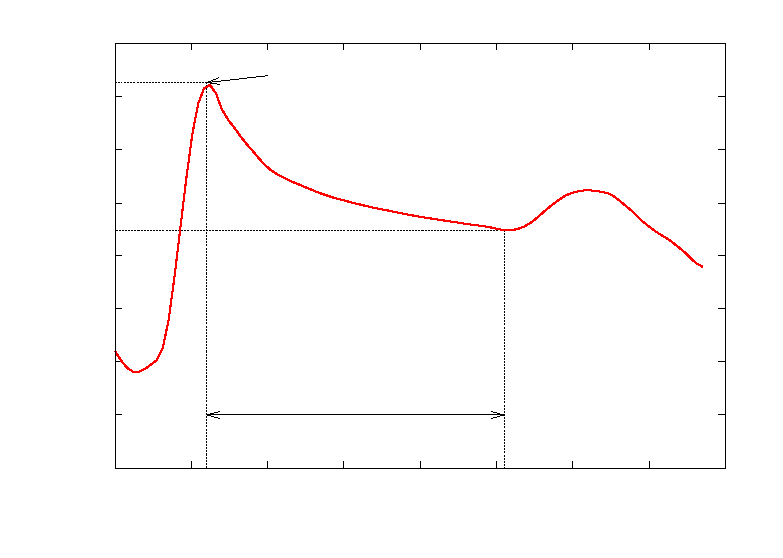
\includegraphics{src/example/hakee}}%
    \gplfronttext
  \end{picture}%
\endgroup

    \end{center}
    \caption{CPVC 转矩-时间 曲线示例图}
    \label{figExHakee}
\end{figure}

\subsection{静态热稳定性}
CPVC 配混料在加工或再加工过程都会在较高温度的设备中停留一定时间,CPVC 制品在使用过程中也会经受一定的环境温度,这就要求热稳定剂能赋予 CPVC 以合适的静态热稳定性。根据 CPVC 热分解导致物料颜色变化或释放出氯化氢的特征,建立了变色法和脱氯化氢法两类评价静态热稳定性的方法。本实验采用变色法\footnote{执行标准 GB/T 9349—2002《聚氯乙烯、相关含氯均聚物和共聚物及其共混物热稳定性的测定 变色法》}进行 CPVC 静态热稳定性的表征。\par
烘箱法:将边长 15 mm,厚度约 1 mm 的正方形试样,放在平铺于架子上的新的干净铝箔上面,在强制鼓风烘箱中于高温下加热不同时间。每隔一定时间取出一片试样,从测试开始至最初观察到颜色变化即为初期热稳定定性,从测试开始至试样完全变黑的时间则为长期热稳定性。

\subsection{玻璃化转变温度}
本实验中采用 DMA 对玻璃化转变温度进行测试。DMA 是对试样施加恒定振幅的正弦交变应力,观察应变随温度或时间的变化规律,从而计算力学参数用以表征材料粘弹性的一种试验方法。在聚合物玻璃化转变过程中,其粘弹性有很大改变,从而可用 DMA 测定 $T_g$。DMA 曲线通常有储能模量、损耗模量、损耗因子这三个信号,对应的 $T_g$ 也可有三种取法,分别为储能模量的台阶式下降曲线部分的起始点、损耗模量的峰值温度、损耗因子\footnote{损耗角正切:$tan \, \delta = \frac{G''}{G'}$}的峰值温度。本实验取损耗因子的峰值温度作为最终测试得到的玻璃化转变温度。如图 \ref{figExTg} 所示,在加热过程中,样品的损耗因子出现了一个峰值,取峰值所在温度为样品的玻璃化转变温度。

\begin{figure}[!htbp]
    \begin{center}
        % GNUPLOT: LaTeX picture with Postscript
\begingroup
  \makeatletter
  \providecommand\color[2][]{%
    \GenericError{(gnuplot) \space\space\space\@spaces}{%
      Package color not loaded in conjunction with
      terminal option `colourtext'%
    }{See the gnuplot documentation for explanation.%
    }{Either use 'blacktext' in gnuplot or load the package
      color.sty in LaTeX.}%
    \renewcommand\color[2][]{}%
  }%
  \providecommand\includegraphics[2][]{%
    \GenericError{(gnuplot) \space\space\space\@spaces}{%
      Package graphicx or graphics not loaded%
    }{See the gnuplot documentation for explanation.%
    }{The gnuplot epslatex terminal needs graphicx.sty or graphics.sty.}%
    \renewcommand\includegraphics[2][]{}%
  }%
  \providecommand\rotatebox[2]{#2}%
  \@ifundefined{ifGPcolor}{%
    \newif\ifGPcolor
    \GPcolorfalse
  }{}%
  \@ifundefined{ifGPblacktext}{%
    \newif\ifGPblacktext
    \GPblacktexttrue
  }{}%
  % define a \g@addto@macro without @ in the name:
  \let\gplgaddtomacro\g@addto@macro
  % define empty templates for all commands taking text:
  \gdef\gplbacktext{}%
  \gdef\gplfronttext{}%
  \makeatother
  \ifGPblacktext
    % no textcolor at all
    \def\colorrgb#1{}%
    \def\colorgray#1{}%
  \else
    % gray or color?
    \ifGPcolor
      \def\colorrgb#1{\color[rgb]{#1}}%
      \def\colorgray#1{\color[gray]{#1}}%
      \expandafter\def\csname LTw\endcsname{\color{white}}%
      \expandafter\def\csname LTb\endcsname{\color{black}}%
      \expandafter\def\csname LTa\endcsname{\color{black}}%
      \expandafter\def\csname LT0\endcsname{\color[rgb]{1,0,0}}%
      \expandafter\def\csname LT1\endcsname{\color[rgb]{0,1,0}}%
      \expandafter\def\csname LT2\endcsname{\color[rgb]{0,0,1}}%
      \expandafter\def\csname LT3\endcsname{\color[rgb]{1,0,1}}%
      \expandafter\def\csname LT4\endcsname{\color[rgb]{0,1,1}}%
      \expandafter\def\csname LT5\endcsname{\color[rgb]{1,1,0}}%
      \expandafter\def\csname LT6\endcsname{\color[rgb]{0,0,0}}%
      \expandafter\def\csname LT7\endcsname{\color[rgb]{1,0.3,0}}%
      \expandafter\def\csname LT8\endcsname{\color[rgb]{0.5,0.5,0.5}}%
    \else
      % gray
      \def\colorrgb#1{\color{black}}%
      \def\colorgray#1{\color[gray]{#1}}%
      \expandafter\def\csname LTw\endcsname{\color{white}}%
      \expandafter\def\csname LTb\endcsname{\color{black}}%
      \expandafter\def\csname LTa\endcsname{\color{black}}%
      \expandafter\def\csname LT0\endcsname{\color{black}}%
      \expandafter\def\csname LT1\endcsname{\color{black}}%
      \expandafter\def\csname LT2\endcsname{\color{black}}%
      \expandafter\def\csname LT3\endcsname{\color{black}}%
      \expandafter\def\csname LT4\endcsname{\color{black}}%
      \expandafter\def\csname LT5\endcsname{\color{black}}%
      \expandafter\def\csname LT6\endcsname{\color{black}}%
      \expandafter\def\csname LT7\endcsname{\color{black}}%
      \expandafter\def\csname LT8\endcsname{\color{black}}%
    \fi
  \fi
    \setlength{\unitlength}{0.0500bp}%
    \ifx\gptboxheight\undefined%
      \newlength{\gptboxheight}%
      \newlength{\gptboxwidth}%
      \newsavebox{\gptboxtext}%
    \fi%
    \setlength{\fboxrule}{0.5pt}%
    \setlength{\fboxsep}{1pt}%
\begin{picture}(7200.00,5040.00)%
    \gplgaddtomacro\gplbacktext{%
      \csname LTb\endcsname%
      \put(814,704){\makebox(0,0)[r]{\strut{}$0$}}%
      \put(814,1518){\makebox(0,0)[r]{\strut{}$0.2$}}%
      \put(814,2332){\makebox(0,0)[r]{\strut{}$0.4$}}%
      \put(814,3147){\makebox(0,0)[r]{\strut{}$0.6$}}%
      \put(814,3961){\makebox(0,0)[r]{\strut{}$0.8$}}%
      \put(814,4775){\makebox(0,0)[r]{\strut{}$1$}}%
      \put(946,484){\makebox(0,0){\strut{}$40$}}%
      \put(1678,484){\makebox(0,0){\strut{}$60$}}%
      \put(2410,484){\makebox(0,0){\strut{}$80$}}%
      \put(3142,484){\makebox(0,0){\strut{}$100$}}%
      \put(3875,484){\makebox(0,0){\strut{}$120$}}%
      \put(4607,484){\makebox(0,0){\strut{}$140$}}%
      \put(5339,484){\makebox(0,0){\strut{}$160$}}%
      \put(6071,484){\makebox(0,0){\strut{}$180$}}%
      \put(6803,484){\makebox(0,0){\strut{}$200$}}%
      \put(1078,4266){\makebox(0,0)[l]{\strut{}$tan \, \delta$ maximun}}%
      \put(4988,924){\rotatebox{90}{\makebox(0,0)[l]{\strut{}$T_g$}}}%
    }%
    \gplgaddtomacro\gplfronttext{%
      \csname LTb\endcsname%
      \put(176,2739){\rotatebox{-270}{\makebox(0,0){\strut{}损耗因子}}}%
      \put(3874,154){\makebox(0,0){\strut{}温度/\cd}}%
    }%
    \gplbacktext
    \put(0,0){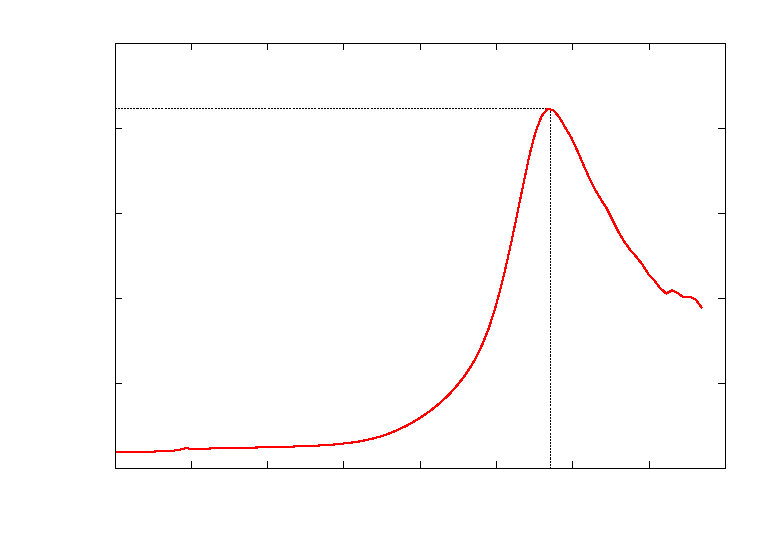
\includegraphics{src/example/tg}}%
    \gplfronttext
  \end{picture}%
\endgroup

    \end{center}
    \caption{CPVC DMA 损耗因子-温度 曲线示例图}
    \label{figExTg}
\end{figure}

\subsection{维卡软化点}
维卡软化点是将热塑性塑料置于特定液体传热介质中,在一定的负荷、一定的等速升温条件下,测定试样被 1 $\rm{mm^2}$ 针头压入 1 mm 时的温度\footnote{执行标准 GB 1633-1979}。实验测得的维卡软化点适用于控制质量和作为衡量材料热性能的一个指标,但不代表材料的使用温度。

\subsection{拉伸强度}
拉伸强度定义为断裂前试样所能承受的最大应力,单位为 MPa,用来评价材料的抗拉性能。拉伸强度的计算公式见式 \eqref{eqTenS},其中 $P$ 为样品承受的最大载荷,$b$ 和 $d$ 分别为试样的宽度和厚度。

\begin{equation}
    \label{eqTenS}
    \sigma_t = \frac{P}{bd}
\end{equation}

本实验中采用万能试验机进行拉伸强度测试\footnote{执行标准 GB/T 1040.2-2006},设置拉伸速率为 10 mm/min,夹具距离为 80 mm,样条的最窄宽度为 6 mm,厚度为 4 mm。

\subsection{弯曲强度}
弯曲强度是指材料在弯曲负荷作用下破裂或达到规定弯矩时能承受的最大应力,此应力为弯曲时的最大正应力,以 MPa 为单位。它反映了材料抗弯曲的能力,用来评价材料的弯曲性能。横力弯曲时,弯矩 M 随截面位置变化,一般情况下,最大正应力 $\sigma_{max}$ 发生于弯矩最大的截面上,且离中性轴最远处。因此,最大正应力不仅与弯矩 M 有关,还与截面形状和尺寸有关。最大正应力计算公式见式 \eqref{eqBendS},其中 $\sigma_{max}$ 为最大弯矩,$W$ 为抗弯截面系数。

\begin{equation}
    \label{eqBendS}
    \sigma_{max} = \frac{M_{max}}{W}
\end{equation}

本实验同样使用万能试验机进行弯曲强度测试\footnote{执行标准 GB/T 9341-2008},设置移动速率为 2 mm/min,样条尺寸为 80 mm$\times$10 mm$\times$4 mm,跨度为 64 mm。

\subsection{缺口冲击强度}
冲击强度是材料在受到冲击后断裂吸收冲击能量的能力,用于评价材料的抗冲击能力或判断材料的脆性和韧性程度。缺口冲击强度的计算公式见式 \eqref{eqImpactS},其中 $aiN$ 为缺口冲击强度(Izod impact strength of a notched specimen),$x\%$ 为实验测得百分比,$S$ 为缺口处截面面积。

\subsection{SEM 观测冲击断裂面样貌}


\begin{equation}
    \label{eqImpactS}
    aiN = (\frac{2.57 J \times x\%}{S}) KJ/m^2
\end{equation}

本实验采用落锤冲击强度仪进行缺口冲击强度测试\footnote{执行标准 ISO 180/1A},缺口形状为“V”形,深度为 2 mm,落锤满载能量为 2.75 J。
